\documentclass[aps,prb,amsfonts,amsmath,amssymb,showpacs,groupedaddress,superscriptaddress]{revtex4-1}
\usepackage{bm}
\usepackage{color}
\usepackage{graphicx}
\usepackage[colorlinks,urlcolor=blue,linkcolor=blue,anchorcolor=blue,citecolor=blue,bookmarks]{hyperref}

\begin{document}

\title{Artificial two-dimensional Mott insulating superstructures with a large Mott gap: Theoretical Part}

\date{\today}

\maketitle

To have a better understading of the experimental observations, we construct single-band Hubbard model with renormalized hopping coefficients to describe these systems and calculate the local density of states by using cluster perturbation theory (CPT)~\cite{PhysRevB.48.418,PhysRevLett.84.522}.

For the $(3\sqrt{7} \times 3\sqrt{7})R19.1^\circ$ surface (referred to as Phase 1 in the following), the corresponding proposed atomic structural is shown in Fig.~\ref{fig:STMTopographicImage}(g). The unit cell contains twenty-three sites while three of them are somewhat isolated, i.e., the three blue circles are speparated from the others. Considering that the hopping amplitude is inversely proportional to the square of the distance, it is reasonable to neglect the three isolated sites in a simplified model. We only include these hopping terms shown in Fig.~\ref{fig:ModelForPhase1} and the resulting Hamiltonian takes the following form:
\begin{equation}
    H = -\sum_{i,j,\sigma} t_{ij}(c_{i\sigma}^{\dagger}c_{j\sigma} + \text{H.c.}) + U \sum_{i} n_{i\uparrow} n_{i\downarrow}
    \label{eq:ModelHamiltonian}
\end{equation}
where $t_{ij}$ is the effective hopping amplitude and $U$ the effective on-site Coulomb repulsion. In Fig.~\ref{fig:ModelForPhase1}, the red points correspond to the center brightest spots in Fig.~\ref{fig:STMTopographicImage}(d), and the blue points correspond to the surrounding less bright spots in Fig.~\ref{fig:STMTopographicImage}(d). The hopping amplitudes between the center red point and the surrounding blue points are taken to be $t_0$, and the hopping amplitudes between these adjacent blue points are $t_1$. Since the atoms corresponding to the brightest spots in the center are not in the same atomic layer as the atoms corresponding to the less bright spots around (see Fig.~\ref{fig:STMTopographicImage}(d)), $t_0$ should be less than $t_1$. Here, we take $t_0 = 0.5$ and $t_1 = 1.0$.

For this model Hamiltonian, we first consider the non-interacting case (\textit{i.e.,} $U = 0$) which can be diagonalized exactly. The averaged DOS and representative LDOS are shown in Fig.~\ref{fig:TBAForPhase1}. It can be seen from the averaged DOS that the system has an energy gap of $\sim 0.3 t_{1}$. However, the LDOS varies from site to site. For instance, the LDOS of the site labeled as ``0'' is quite different from the sites labeled as ``1'' and ``3''. Especially, the energy gap at the zeroth site is $\sim 3.4 t_{1}$, and yet that at other sites is $\sim 0.3 t_{1}$. This inhomogeneous LDOS is obviously contradictory to the experimental uniform insulating gap. We further include on-site Coulomb repulsion and use CPT to calculate the LDOS. The evolution of the averaged DOS with U is shown in Fig.~\ref{fig:CPTForPhase1}. The energy gap becomes gradually decreased when taking into account of Hubbard-$U$ and a transition from band insulator to metal is identified at $U \approx 3.0 t_{1}$. As we further increase $U$, an energy gap is reopened, indicating a metal-insulator transition. The including of $U = 6 t_{1}$ leads to a large energy gap of $\sim 2.32 t_{1}$ which is comparable with the experimental energy gap of $\sim 2.5 \text{eV}$ if we take $t_{1} = 1\text{eV}$.

\textcolor{red}{We further explored the corresponding LDOS and found that the energy gap is uniform at each lattice sites from 0 to 19 (see Fig.~\ref{fig:CPTForPhase1LDOS}), which is consistent with the experimentally observed homengeneous dI/dV spectra. The agreement between the experimental observation and theoretical calculation indicates the Mott origin of the large energy gap of $\sim 2.5\text{eV}$ for $(3\sqrt{7} \times 3\sqrt{7})R19.1^\circ$ surface.}

For $(\sqrt{133} \times 4\sqrt{3})$ and $(13 \times 13)$ surfaces (referred to as Phase 2 and Phase 3 respectively), we similarly constructed the simplified model for theoretical calculations. Considering the substrate Si atoms form triangular lattice and the surface Sn atoms form well-ordered superstructures, we constructed Hubbard model on triangular lattice with renormalized hopping amplitudes between nearest neighbors to describe Phase 2 and Phase 3. The corresponding tight-bingding model is shown in Fig.~\ref{fig:ModelForPhase2andPhase3}. The points connected by solid red bonds correspond to the bright spots in Fig.~\ref{fig:STMTopographicImage}(e) and (f) and other points correspond to these less bright spots. The hopping amplitudes are $t_{0}$ for these solid red bonds and $t_{1}$ for these dashed green and gray dotted bonds. We assume $t_{0}$ to be greater than $t_{1}$ since these bright spots are on the same atomic layer and connected tighter. Here we take $t_{0} = 1.0$ and $t_{1} = 0.5$. For the non-interacting part, the unit cell contains even number of electrons at half-filling and the system is in metalic state. The calculated averaged DOS as well as local density of states for those non-equivalent sites are shown in Fig.~\ref{fig:TBAForPhase2AndPhase3}. It can be clearly seen from Fig.~\ref{fig:TBAForPhase2AndPhase3} that the local density fo states are homengeneous. We further calculate the DOS of the corresponding Hubbard model by using CPT and the evolution of DOS with Hubbard-$U$ is shown in Fig.~\ref{fig:CPTForPhase2andPhase3}. With the inclusion of Hubbard-$U$, the system undergoes an metal-insulator transition at $U \approx 3 t_{0}$. When we further increase $U$ to $6 t_{0}$ to be consistent with the value of Phase 1, the Mott gap is about $2.84 t_{0}$. The calculated gap size of Phase 2 and Phase3 is larger than the gap size of Phase 1, which is qualitatively consistent the experimental onservation.


\begin{figure}[p]
    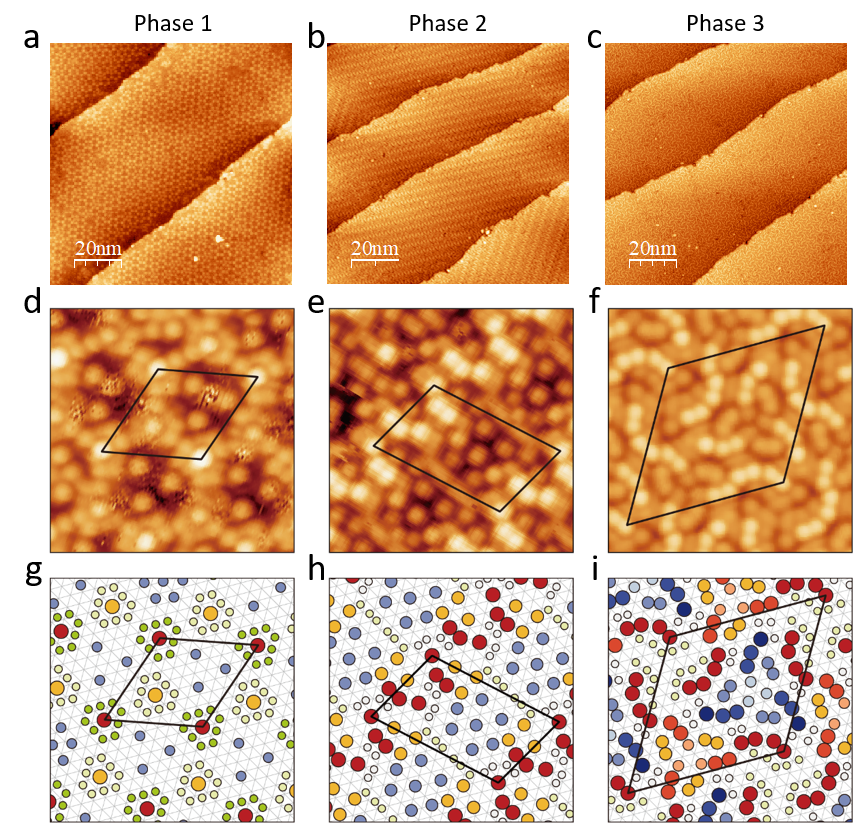
\includegraphics[width=0.80\columnwidth]{fig/STMTopographicImage.png}
    \caption{\label{fig:STMTopographicImage}(Color online) STM characterization of three new superstructures of Sn sub-monolayers on Si(111). (a)-(c) Large-scale STM image (size: 100 $\times$ 100 nm$^2$) taken on $(3\sqrt{7} \times 3\sqrt{7})R19.1^\circ$, $(\sqrt{133} \times 4\sqrt{3})$, and $(13 \times 13)$ surfaces. They are taken at $U = +3.5V$, $U = -2V$, and $U = -2V$ ($I_{t} = 100pA$) respectively. (d)-(f) The atomically resolved STM images of them taken at $U = -2V, I_{t} = 200pA$. The surface unit cells of them are marked in black parallelogram. (g)-(i) The corresponding proposed atomic structural models. The marked surface unit cells in (g)-(i) are the same as these in (d)-(f).}
\end{figure}

\begin{figure}[p]
    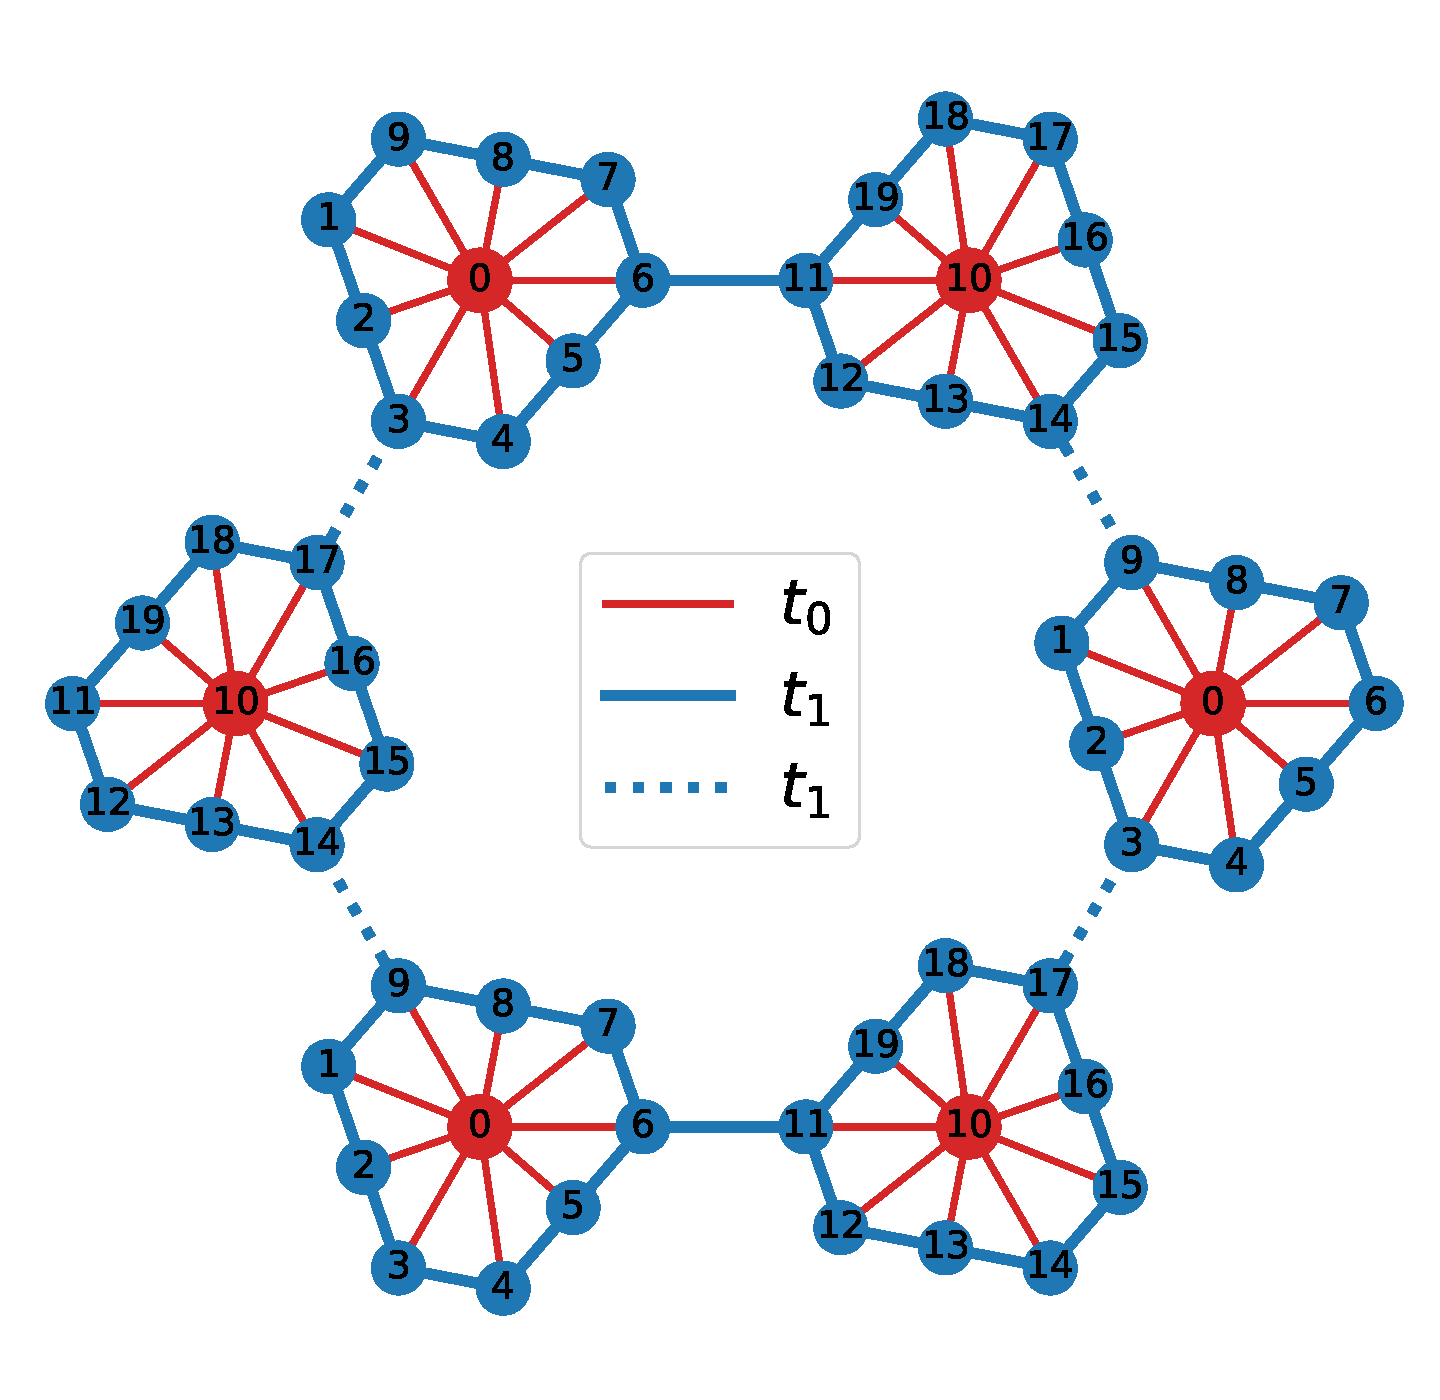
\includegraphics[width=0.80\columnwidth]{fig/ModelForPhase1.pdf}
    \caption{\label{fig:ModelForPhase1} (Color online) Demonstration of the hopping terms for Phase 1. The unit cell has twenty sites labeled from 0 to 19. The soild and dashed lines correspond to the hopping terms $t_{ij} (c_{i\sigma}^{\dagger} c_{j\sigma} + \text{H.c.})$.}
\end{figure}

\begin{figure}[p]
    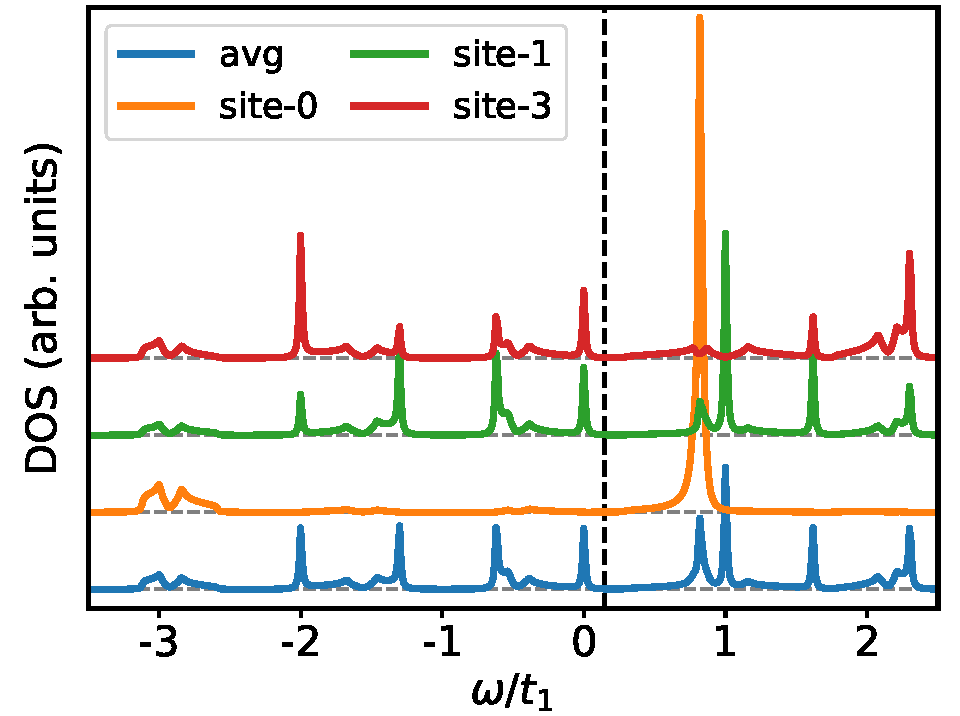
\includegraphics[width=0.5\columnwidth]{fig/TBAForPhase1.pdf}
    \caption{\label{fig:TBAForPhase1} (Color online) Local density of states calculated from the tight-binding model defined in Fig.~\ref{fig:ModelForPhase1}. The blue line is the average of the LDOS over the twenty sites in a unit cell. LDOS for site \{0, 10\}, \{3, 6, 9, 11, 14, 17\}, \{1, 2, 4, 5, 7, 8, 12, 13, 15, 16, 18, 19\} are the same. The black dashed vertical line marks the Fermi energy $E_{F}$.}
\end{figure}

\begin{figure}[p]
    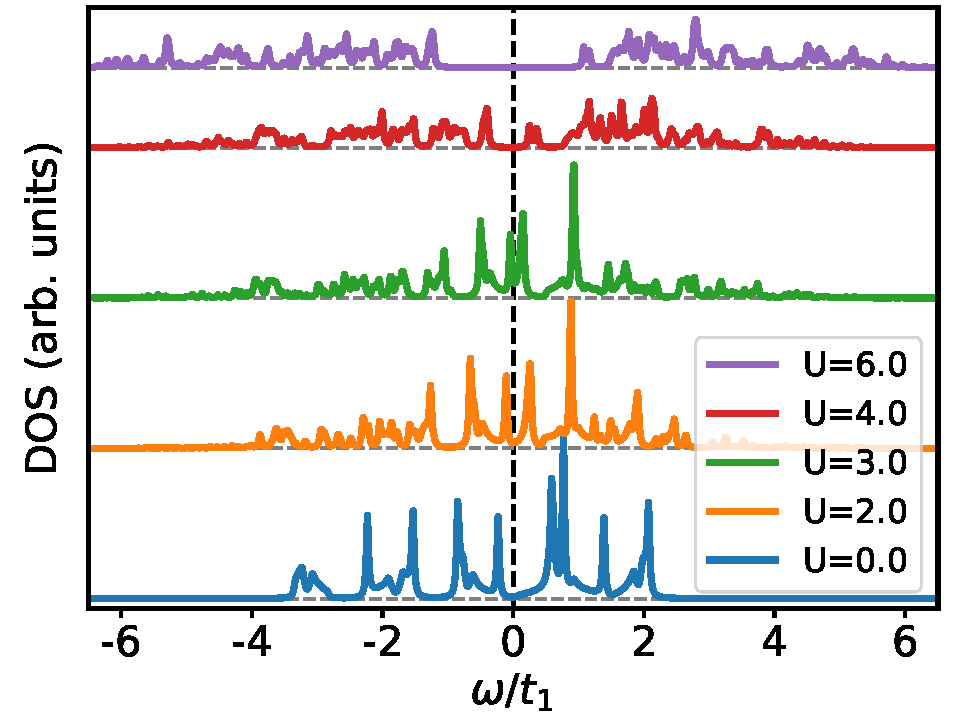
\includegraphics[width=0.5\columnwidth]{fig/CPTForPhase1.pdf}
    \caption{\label{fig:CPTForPhase1} (Color online) The evolution of averaged DOS with Hubbard-$U$. $U$ is in the unit of $t_{1}$. The black dashed vertical line marks the Fermi energy $E_{F}$.}
\end{figure}

\begin{figure}[p]
    \centering
    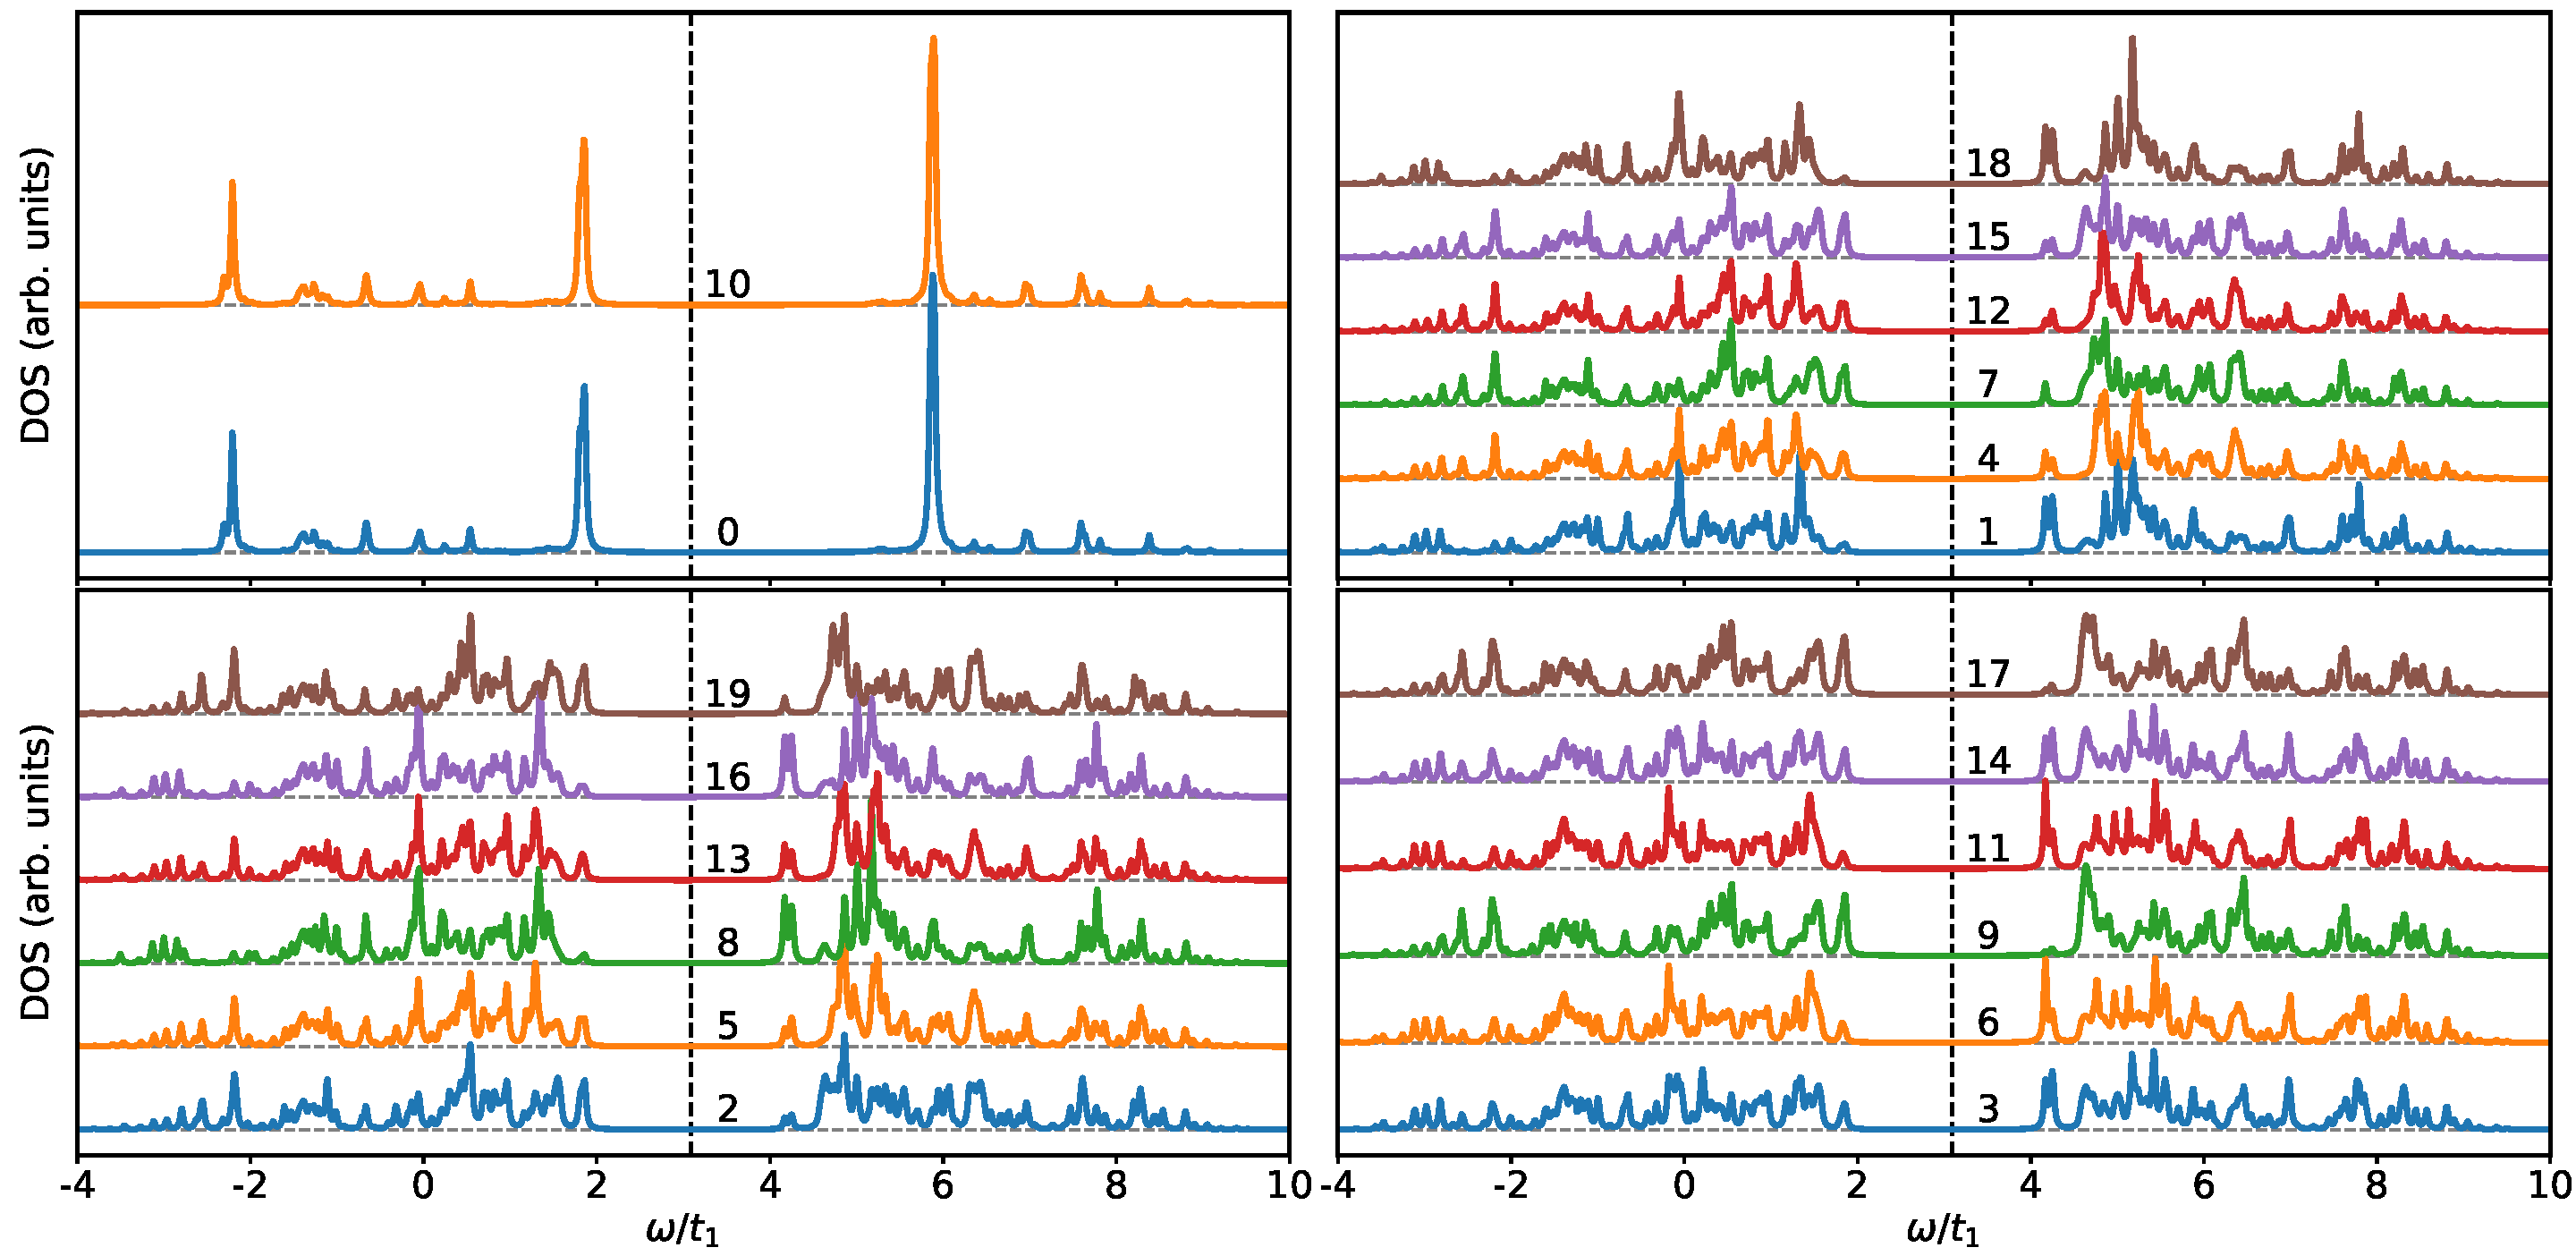
\includegraphics[width=0.95\columnwidth]{fig/CPTForPhase1LDOS.pdf}
    \caption{\label{fig:CPTForPhase1LDOS} (Color online) Local density of states at $U = 6 t_{1}$. The numbers above the curves correspond to the site indices shown in Fig.~\ref{fig:ModelForPhase1}. The black dashed vertical line marks the Fermi energy $E_{F}$.}
\end{figure}

\begin{figure}[p]
    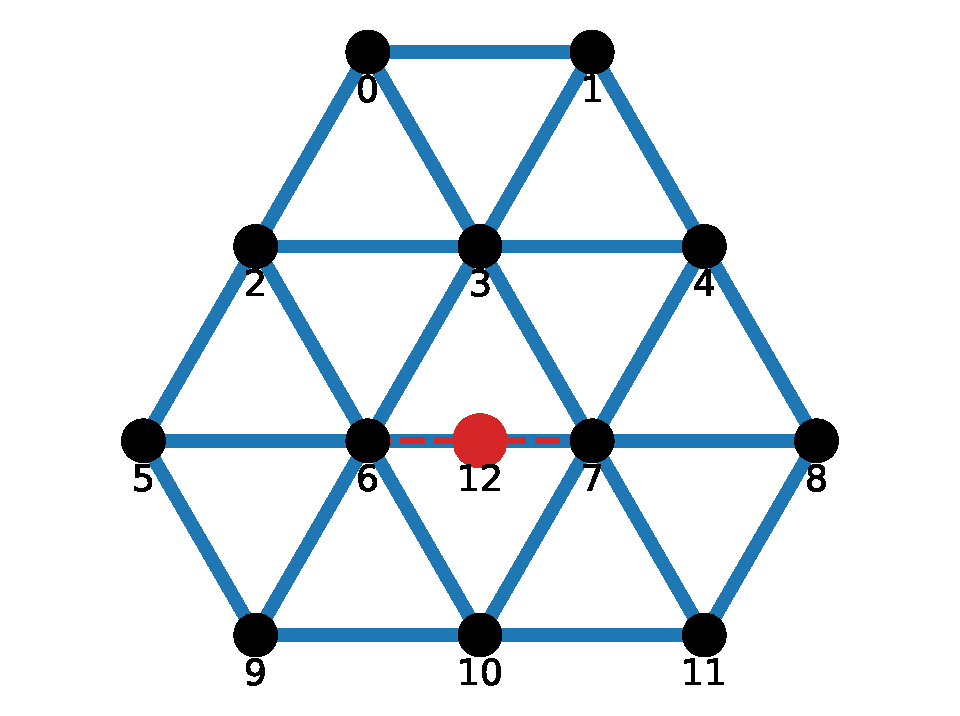
\includegraphics[width=0.5\columnwidth]{fig/ModelForPhase2andPhase3.pdf}
    \caption{\label{fig:ModelForPhase2andPhase3} (Color online) Demonstration of the tight-binding model for Phase 2 and Phase 3. The soild and dashed lines correspond to the hopping terms $t_{ij} (c_{i\sigma}^{\dagger} c_{j\sigma} + \text{H.c.})$.}
\end{figure}

\begin{figure}[p]
    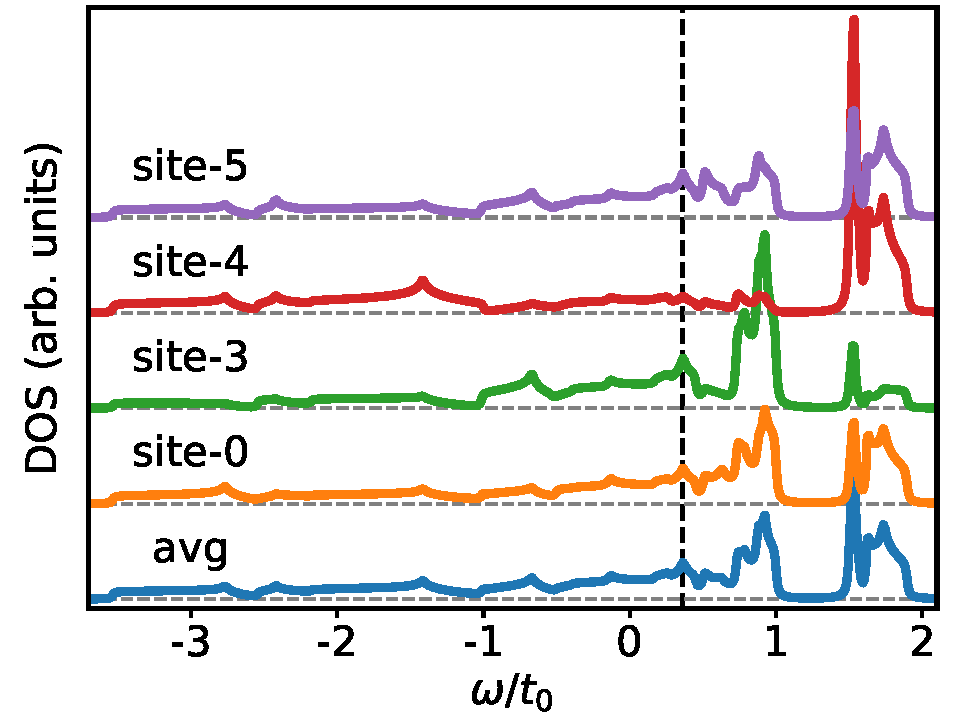
\includegraphics[width=0.5\columnwidth]{fig/TBAForPhase2AndPhase3.pdf}
    \caption{\label{fig:TBAForPhase2AndPhase3} (Color online) Local density of states calculated from the tight-binding model defined in Fig.~\ref{fig:ModelForPhase2andPhase3}. The blue line is the average of the LDOS over the twenty sites in a unit cell. LDOS for site \{0, 1, 2\}, \{3, 6, 9\}, \{4, 7, 10\}, \{5, 8, 11\} are the same. The black dashed vertical line marks the Fermi energy $E_{F}$.}
\end{figure}

\begin{figure}[p]
    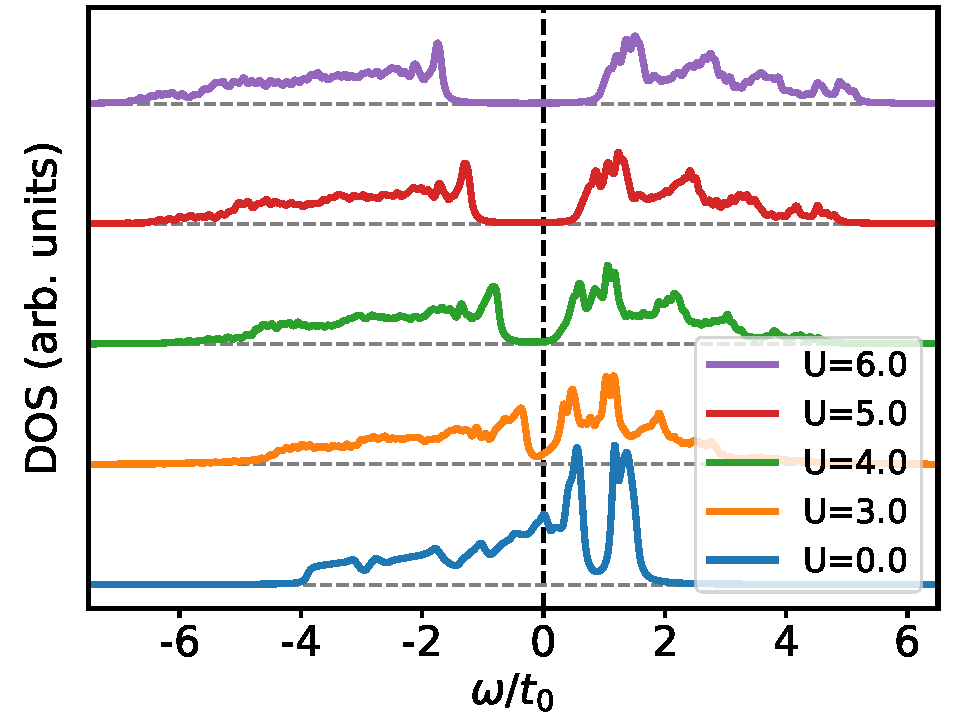
\includegraphics[width=0.5\columnwidth]{fig/CPTForPhase2andPhase3.pdf}
    \caption{\label{fig:CPTForPhase2andPhase3} (Color online) The evolution of averaged DOS with Hubbard-$U$. $U$ is in the unit of $t_{0}$. The black dashed vertical line marks the Fermi energy $E_{F}$.}
\end{figure}

\begin{figure}[p]
    \includegraphics[width=0.95\columnwidth]{fig/CPTForPhase2andPhase3LDOS.pdf}
    \caption{\label{fig:CPTForPhase2andPhase3LDOS} Local density of states at $U = 6 t_{0}$. The numbers above the curves correspond to the site indices shown in Fig.~\ref{fig:ModelForPhase2andPhase3}. The black dashed vertical line marks the Fermi energy $E_{F}$.}
\end{figure}

\bibliography{TheoreticalFormalism}

\end{document}
